\section{Introdução}\label{introduuxe7uxe3o}

A evolução dos computadores fez com que mais formas diferentes de acesso
a informação sejam possíveis. Hoje em dia é possível, por exemplo,
verificar sua conta de \emph{e-mail} de seu computador pessoal, ou de
seu \emph{notebook}, de seu aparelho celular ou ainda de seu
\emph{smartwatch}. Cada um desses aparelhos com diferentes tamanhos
físicos e diferentes poderes de processamento. Nesse cenário, voltamos
um pouco da ideia de \emph{Mainframes} para acesso remoto de arquivos ou
serviços, mas agora com novas estruturas e arquiteturas, que ficou
conhecido como Nuvem.

Para atender a estes diversos tipos de dispositivos citados acima que
acessam os mesmos recursos surge o conceito de Serviços. O que se propõe
é tornar o servidor e o cliente independentes, para que seja possível
ter acesso aos mesmos recursos do servidor de vários clientes
diferentes.

\section{Definição}\label{definiuxe7uxe3o}

Em 2000, surge o conceito do REST (do inglês \emph{Representational
State Transfer}) criado por Roy Thomas Fielding em sua dissertação de
Doutorado. Uma dos pontos-chave deste conceito é desacoplar a interface
de usuário do armazenamento de dados, o que melhoraria a portabilidade
da interface de usuário para múltiplas plataformas \cite{rest:2000}.
Esse padrão se popularizou graças a adoção por empresas como o
\emph{Twitter} em 2006, que fornecedia uma API (do inglês
\emph{Application Programming Interface}) para que terceiros pudessem
fazer algum tipo de integração, como por exemplo \emph{login} com a
conta do \emph{Twitter} em seu aplicativo ao invés de criar um sistema
de \emph{login} próprio.

Em 2015, o \emph{Facebook} publica em formato \emph{Open Source} o
GraphQL, definido como uma \emph{query language} (linguagem de consulta)
para \emph{API}'s. Permite que o cliente obtenha os dados de forma
declarativa e hierarquica \cite{graphql:2015}. É um formato que
adapta-se a qualquer banco de dados ou mecanismo de armazenamento, ou
seja, é possível usá-lo para busca de arquivos em um sistema de arquivos
remoto. Possui 3 tipos de operações básicas: \emph{Query} para obtenção
de dados; \emph{Mutation} para alteração de dados; e
\emph{Subscriptions} para notificação em tempo real.

\section{Estilo Arquitetônico e
Arquitetura}\label{estilo-arquitetuxf4nico-e-arquitetura}

\subsection{REST}\label{rest}

Em sistemas REST há série de restrições arquiteturais, tais como:

\begin{itemize}
\itemsep1pt\parskip0pt\parsep0pt
\item
  \textbf{Cliente-Servidor}: separar a interface de usuário da lógica da
  aplicação.
\item
  \textbf{\emph{Stateless}}: a requisição contém informações suficientes
  sobre o cliente para que o servidor entenda a requisição.
\item
  \textbf{\emph{Cacheable}}: requisições devem ser passíveis de serem
  colocadas em \emph{cache}.
\item
  \textbf{Interface Uniforme}: identificação de recursos é feita através
  de URI e sua implementação é feita de forma abstrata da definição da
  interface.
\item
  \textbf{Sistema em Camadas}: um cliente não deverá distinguir se está
  conectado ao servidor final ou a um intermediário.
\end{itemize}

Seu estilo arquitetônico se encaixa em uma arquitetura em camadas.

\begin{figure}[h]
    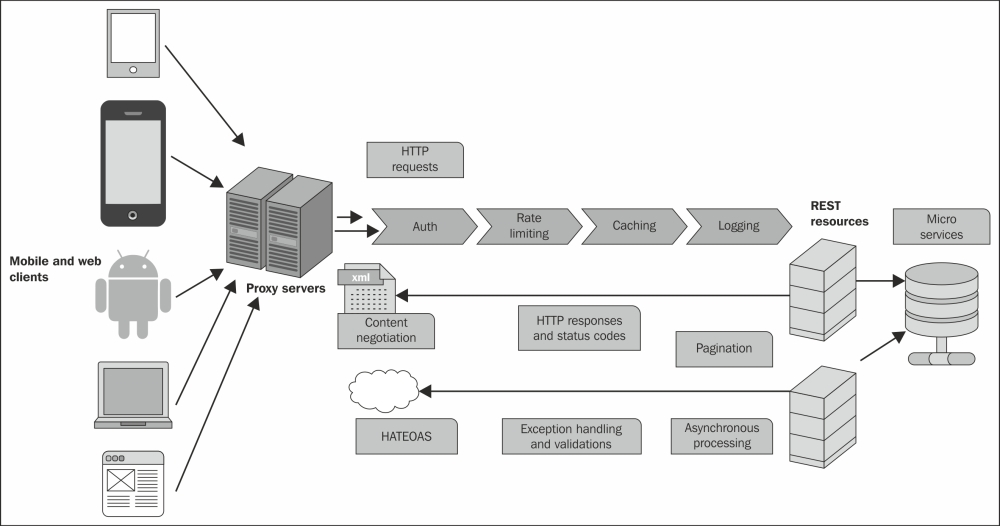
\includegraphics[scale=1.5]{img/rest.jpg}
    \caption{REST}
\end{figure}

\subsection{GraphQL}\label{graphql}

Em sistemas GraphQL podem haver diversos tipos de arquiteturas
diferentes, entre elas:

\begin{itemize}
\itemsep1pt\parskip0pt\parsep0pt
\item
  Servidor GraphQL conectado a um banco de dados, como visto na Figura
  \ref{fig:gql-dbgql-db}.
\item
  Servidor GraphQL atuando como camada intermediária entre sistemas
  legados ou ainda de terceiros integrando-os através de uma únida API
  GraphQL, como visto na Figura \ref{fig:gql-3th-legacy}.
\item
  Uma abordagem híbrida com a junção das 2 abordagem supracitadas, como
  visto na Figura \ref{fig:gql-hybrid}.
\end{itemize}

Seu estilo arquitetônico é híbrido entre arquitetura em camadas e
baseada em eventos, esta última utilizada para notificações em tempo
real.

\begin{figure}[h]
    \centering
    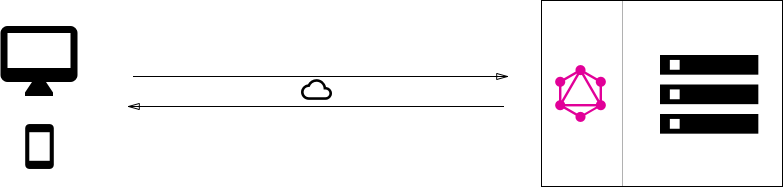
\includegraphics[scale=0.25]{img/gql-db.png}
    \caption{GraphQL com banco de dados}
    \label{fig:gql-dbgql-db}
\end{figure}

\begin{figure}[h]
    \begin{minipage}{.5\textwidth}
        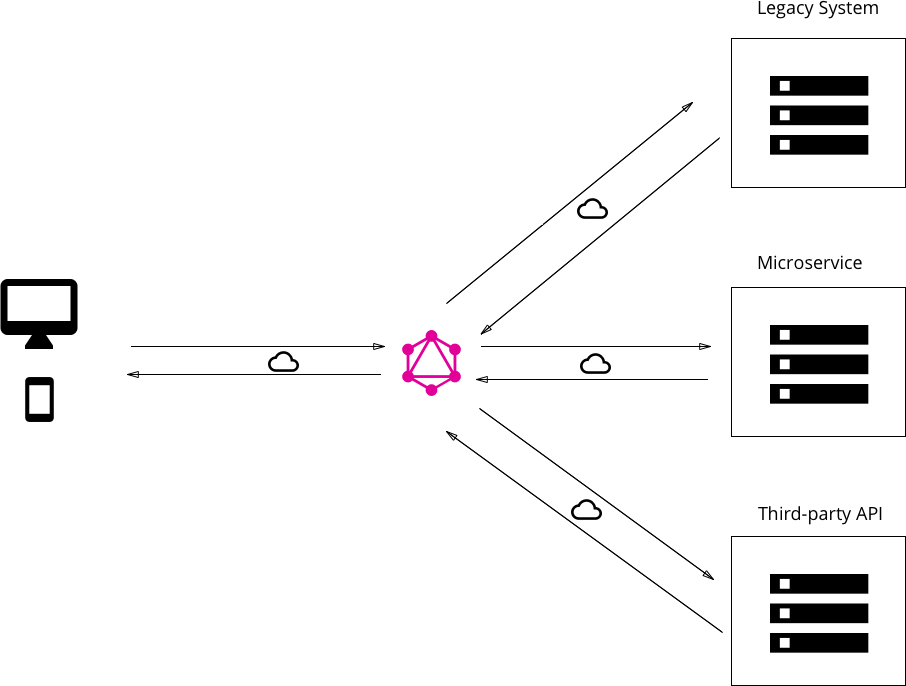
\includegraphics[scale=0.2]{img/gql-3th-legacy.png}
        \caption{GraphQL com sistemas de terceiros ou legados}
        \label{fig:gql-3th-legacy}
    \end{minipage}
    \begin{minipage}{.5\textwidth}
        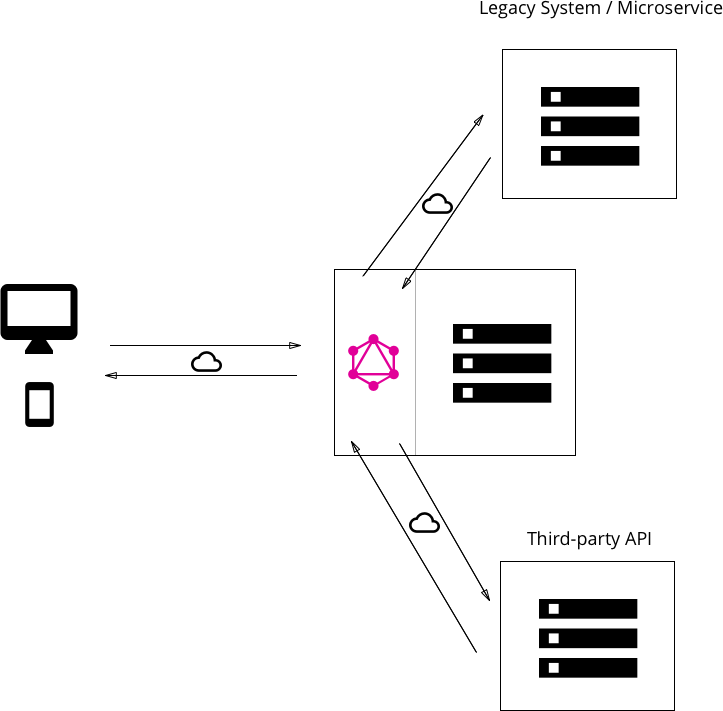
\includegraphics[scale=0.25]{img/gql-hybrid.png}
        \caption{GraphQL híbrido}
        \label{fig:gql-hybrid}
    \end{minipage}
\end{figure}

\section{Comunicação}\label{comunicauxe7uxe3o}

\subsection{REST}\label{rest-1}

A comunicação é feita através do protocolo HTTP, em que é recomendado o
uso explícito dos métodos do HTTP para operações: criar, ler, atualizar
e deletar, como é mostrado a seguir:

\begin{itemize}
\itemsep1pt\parskip0pt\parsep0pt
\item
  Para criar um recurso no servidor, utilize o método \texttt{POST};
\item
  Para resgatar um recurso, use \texttt{GET};
\item
  Para modificar um recurso, use \texttt{PUT};
\item
  Para deletar um recurso, use \texttt{DELETE}.
\end{itemize}

\subsection{GraphQL}\label{graphql-1}

A comunicação pode ser feita por qualquer protocolo, basta que para isso
seja implementado no servidor. A única restrição é que haja somente um
\emph{endpoint} para a conversa entre cliente e servidor.

\section{Nomeação}\label{nomeauxe7uxe3o}

\section{Dificuldades e Soluções}\label{dificuldades-e-soluuxe7uxf5es}

\section{Considerações Finais}\label{considerauxe7uxf5es-finais}
